% Source: graduate-coursework/Research/Intro_to_Agents/handouts/Part6_MultiTier_Architecture.tex

\documentclass[border=4pt]{standalone}
\usepackage{amsmath,amssymb,amsfonts}
\usepackage[T1]{fontenc}
\usepackage{graphicx}
\usepackage{lmodern}
\usepackage{tikz}
\usepackage{xcolor}
\usetikzlibrary{shapes,arrows.meta,positioning,calc,fit,backgrounds,chains,decorations.pathreplacing}

\definecolor{UofSCGarnet}{HTML}{73000a}
\definecolor{UofSCBlack}{HTML}{000000}
\definecolor{UofSCWhite}{HTML}{ffffff}
\definecolor{UofSCRose}{HTML}{CC2E40}
\definecolor{UofSCAtlantic}{HTML}{466A9F}
\definecolor{UofSCCongaree}{HTML}{1F414D}
\definecolor{UofSCHorseshoe}{HTML}{65780B}
\definecolor{UofSCGrass}{HTML}{CED318}
\definecolor{UofSCHoneycomb}{HTML}{A49137}
\definecolor{UofSC90Black}{HTML}{363636}
\definecolor{UofSC70Black}{HTML}{5C5C5C}
\definecolor{UofSC50Black}{HTML}{A2A2A2}
\definecolor{UofSCWarmGrey}{HTML}{676156}
\definecolor{UofSCSandstorm}{HTML}{FFF2E3}
\definecolor{UofSCDarkGarnet}{HTML}{570008}
\definecolor{UofSCAzalea}{HTML}{844247}

\tikzset{
    % Base node style
    basenode/.style={
        draw=UofSCBlack,
        fill=UofSCWhite,
        line width=0.8pt,
        minimum height=0.8cm,
        minimum width=2cm,
        align=center,
        font=\small
    },
    % Strategy layer style
    strategynode/.style={
        basenode,
        fill=UofSCGarnet,
        text=UofSCWhite,
        minimum height=1cm,
        minimum width=4cm
    },
    % Planning layer style
    planningnode/.style={
        basenode,
        fill=UofSCAtlantic,
        text=UofSCWhite,
        minimum height=0.9cm,
        minimum width=3.5cm
    },
    % Execution layer style
    execnode/.style={
        basenode,
        fill=UofSCCongaree,
        text=UofSCWhite,
        minimum height=0.8cm,
        minimum width=2.5cm
    },
    % Generic box
    genericbox/.style={
        basenode,
        minimum width=2.8cm
    },
    % Arrow styles (straight lines only)
    myarrow/.style={
        ->,
        >=Stealth,
        line width=0.8pt,
        draw=UofSCBlack
    },
    % Bidirectional arrow
    biarrow/.style={
        <->,
        >=Stealth,
        line width=0.8pt,
        draw=UofSCBlack
    },
    % Phase box style
    phasebox/.style={
        basenode,
        minimum width=3.5cm,
        minimum height=1.2cm,
        font=\small\bfseries
    },
    % Small box
    smallbox/.style={
        basenode,
        minimum width=1.5cm,
        minimum height=0.6cm,
        font=\scriptsize
    },
    % Leader node
    leadernode/.style={
        basenode,
        fill=UofSCGarnet,
        text=UofSCWhite,
        minimum width=3cm,
        minimum height=1cm
    },
    % Worker node
    workernode/.style={
        basenode,
        fill=UofSC70Black,
        text=UofSCWhite,
        minimum width=1.2cm,
        minimum height=0.7cm,
        font=\scriptsize
    }
}

\begin{document}
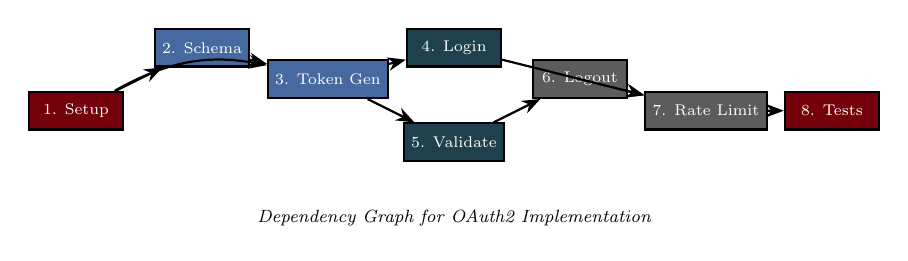
\begin{tikzpicture}[scale=0.8, transform shape]
        % Task nodes
        \node[smallbox, fill=UofSCGarnet, text=white] (t1) at (0,2) {1. Setup};
        \node[smallbox, fill=UofSCAtlantic, text=white] (t2) at (2,3) {2. Schema};
        \node[smallbox, fill=UofSCAtlantic, text=white] (t3) at (4,2.5) {3. Token Gen};
        \node[smallbox, fill=UofSCCongaree, text=white] (t4) at (6,3) {4. Login};
        \node[smallbox, fill=UofSCCongaree, text=white] (t5) at (6,1.5) {5. Validate};
        \node[smallbox, fill=UofSC70Black, text=white] (t6) at (8,2.5) {6. Logout};
        \node[smallbox, fill=UofSC70Black, text=white] (t7) at (10,2) {7. Rate Limit};
        \node[smallbox, fill=UofSCGarnet, text=white] (t8) at (12,2) {8. Tests};

        % Arrows showing dependencies
        \draw[myarrow] (t1) -- (t2);
        \draw[myarrow] (t1) to[bend left=20] (t3);
        \draw[myarrow] (t2) -- (t3);
        \draw[myarrow] (t3) -- (t4);
        \draw[myarrow] (t3) -- (t5);
        \draw[myarrow] (t5) -- (t6);
        \draw[myarrow] (t4) -- (t7);
        \draw[myarrow] (t6) -- (t7);
        \draw[myarrow] (t7) -- (t8);

        % Label
        \node[font=\footnotesize\itshape] at (6,0.3) {Dependency Graph for OAuth2 Implementation};
    \end{tikzpicture}
\end{document}
